\documentclass{article}
\usepackage{graphicx}
\usepackage{ctex}
\title{暑期科研总结}
\author{王文豪}
\date{\today}
\begin{document}
\maketitle
\section{总结}
通过这个夏令营,我学习了有关光通信的一些理论知识,以及如何使用如Overleaf和Zotero等论文编辑和管理软件,还有AI图形软件。接下来,我将分别描述我所学到的内容。
\section{要点}
\subsection{关于硅基调制器}
硅调制器具有超宽带宽、超小尺寸、超大通带以及与互补金属氧化物半导体(CMOS)集成工艺兼容性等优点,满足了未来超高速应用场景对超高速率、高集成度、多波长通信、高热稳定性和晶圆级生产的需求,是硅基光电子领域的重大突破,为高速、短距离数据中心和光通信的应用提供了重要的技术支持。
\\
\noindent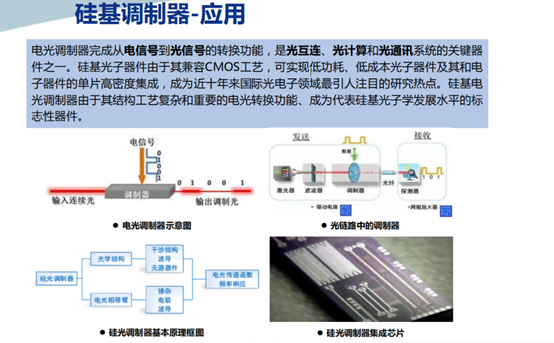
\includegraphics[width=\linewidth]{p1.png}
\noindent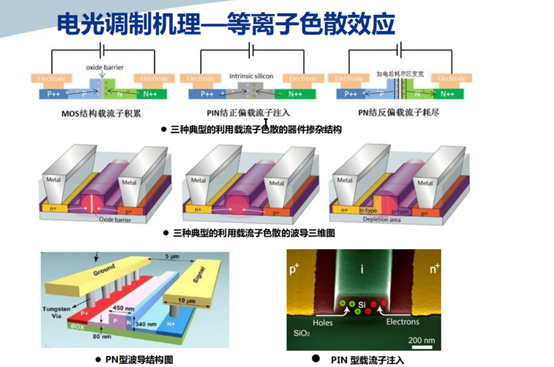
\includegraphics[width=\linewidth]{p2.png}
\newpage
在硅基电子器件的制造过程中,还需要关注蚀刻速率以确保晶圆上均匀雕刻,以及使用离子注入、热扩散和激光掺杂等方法实现均匀掺杂。
\\
\noindent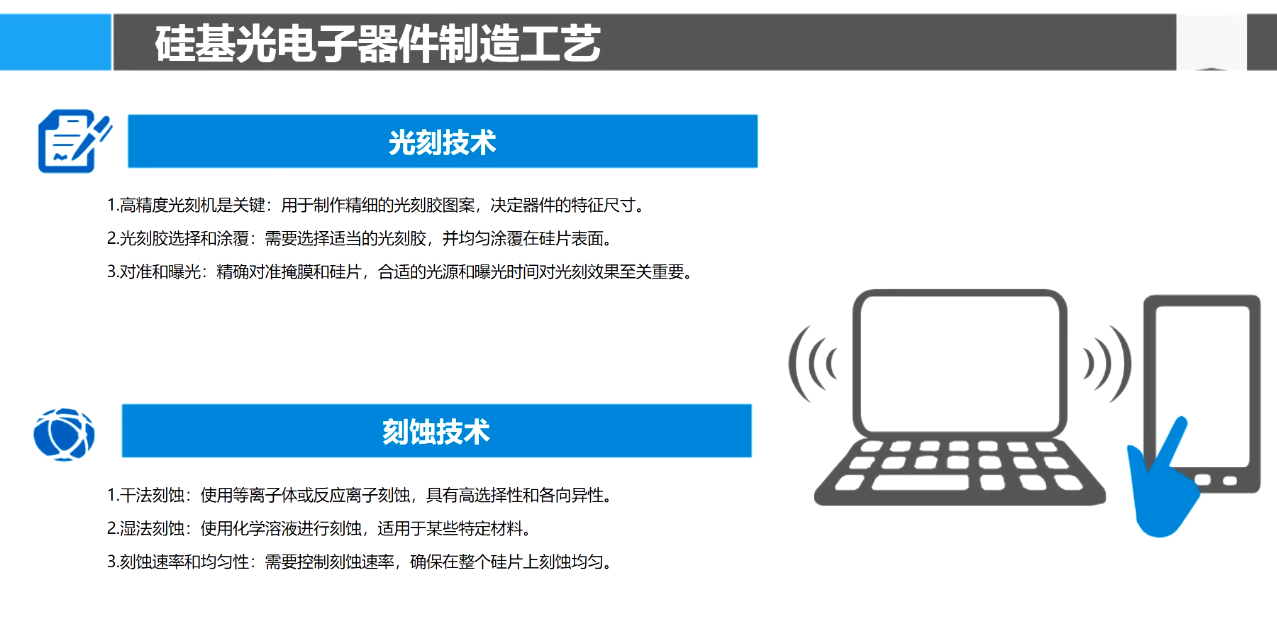
\includegraphics[width=\linewidth]{p3.png}
\subsection{关于使用Overleaf}
在学会使用这个编辑器之前,我一直在使用传统的latex软件进行编辑,但Overleaf让我编辑文档变得更加容易,并为多人共享提供了平台。我最喜欢的功能是可视化编辑功能,它可以将latex复杂的代码转换成可视化界面,这对我编辑和修改文档非常方便。
\\
\noindent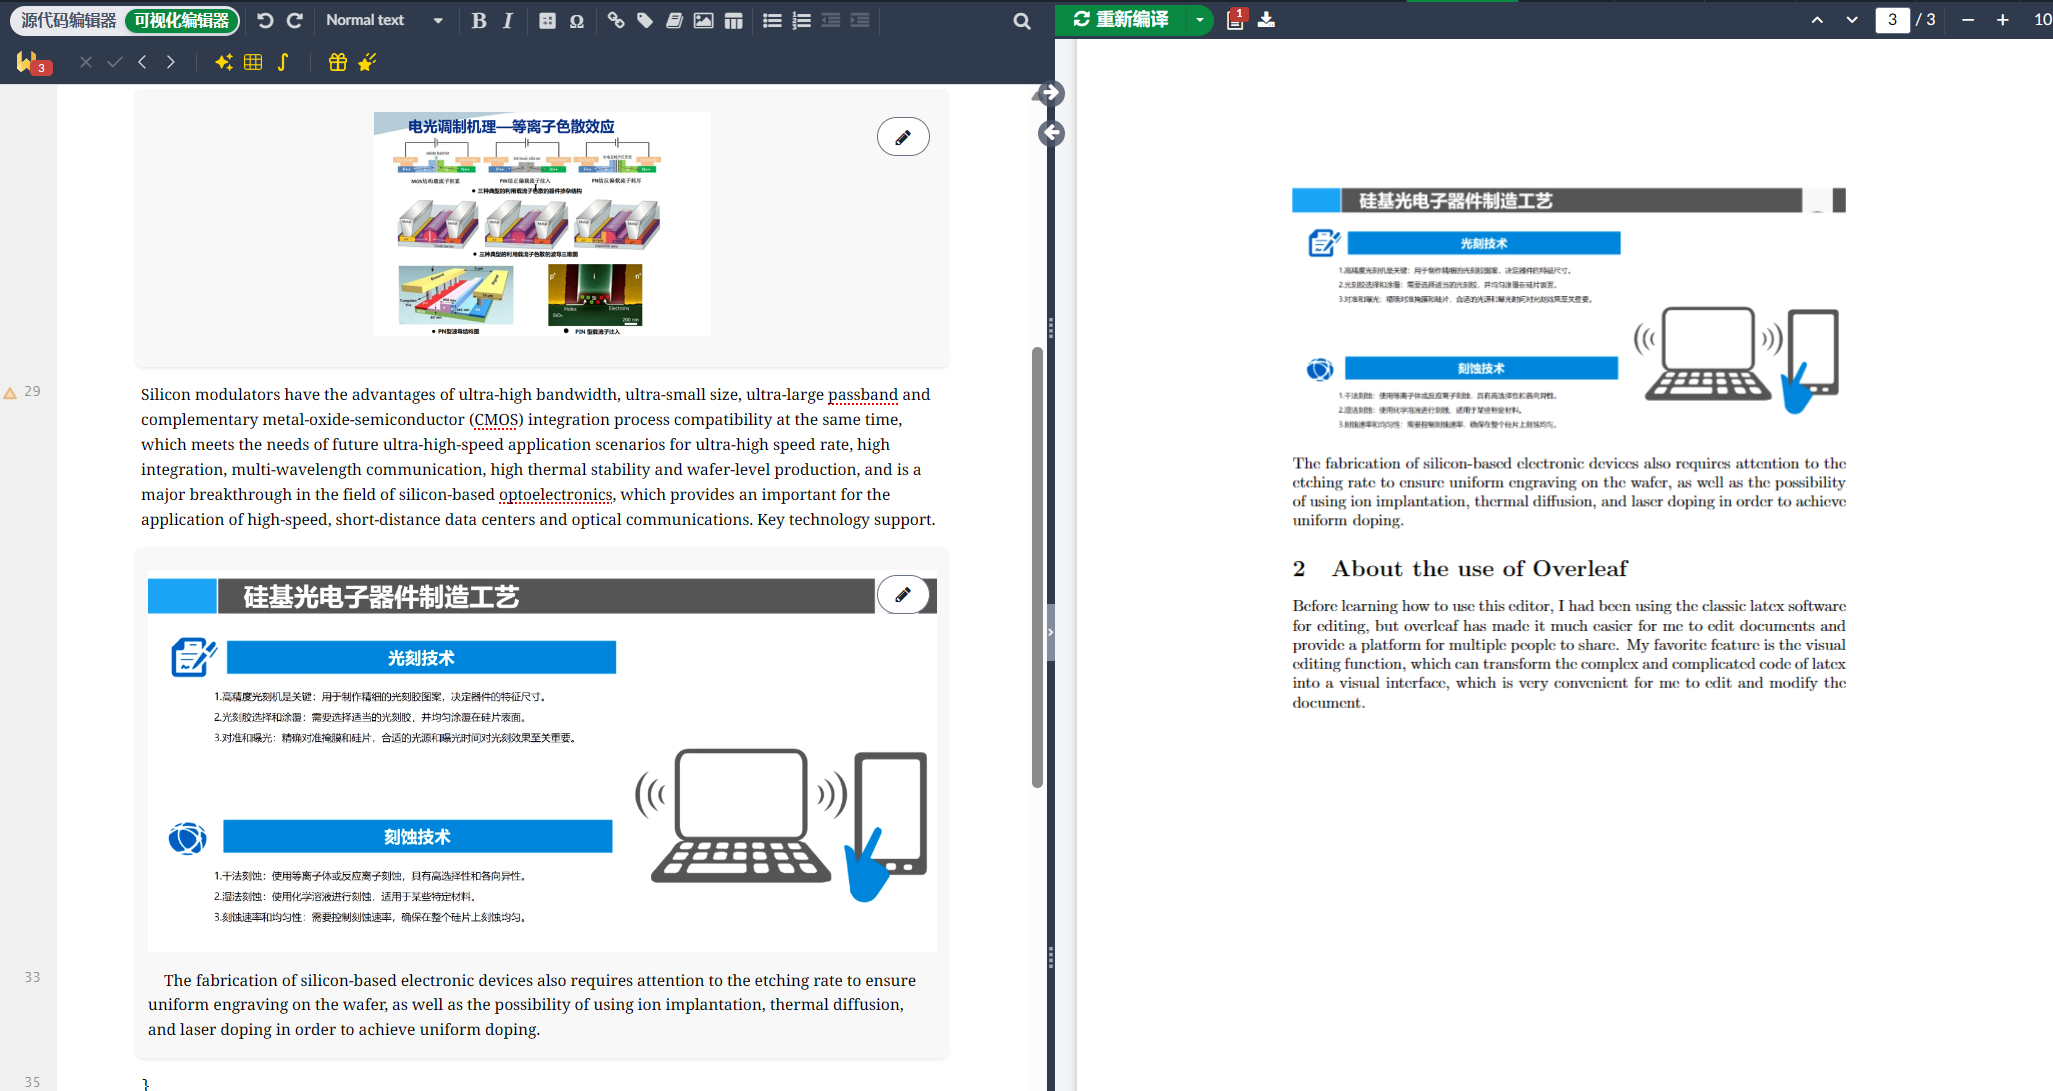
\includegraphics[width=\linewidth]{p4.png}
\subsection{关于使用Zotero}
Zotero在阅读文献时方便我爬取和分类文章,通过清晰地展示文章的标题、摘要和引言,并结合使用NutCloud,我能够更高效地找到和组织我需要的文章。
\\
\noindent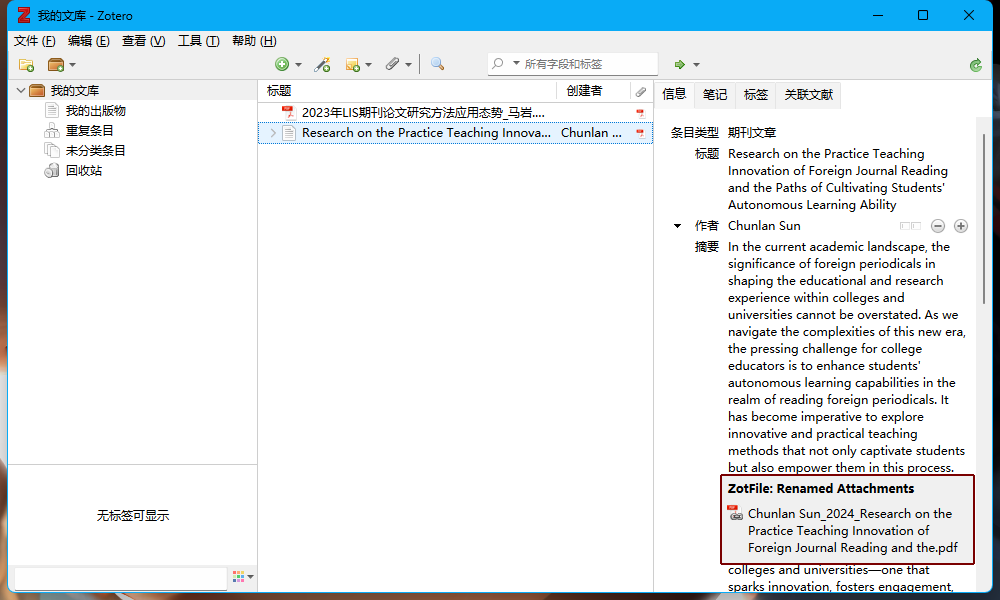
\includegraphics[width=\linewidth]{p5.png}
\subsection{关于使用AI}
我也尝试使用前辈教授的方法绘制连接图,学习Adobe Illustrator的过程让我感到绘图非常方便。
\\
\noindent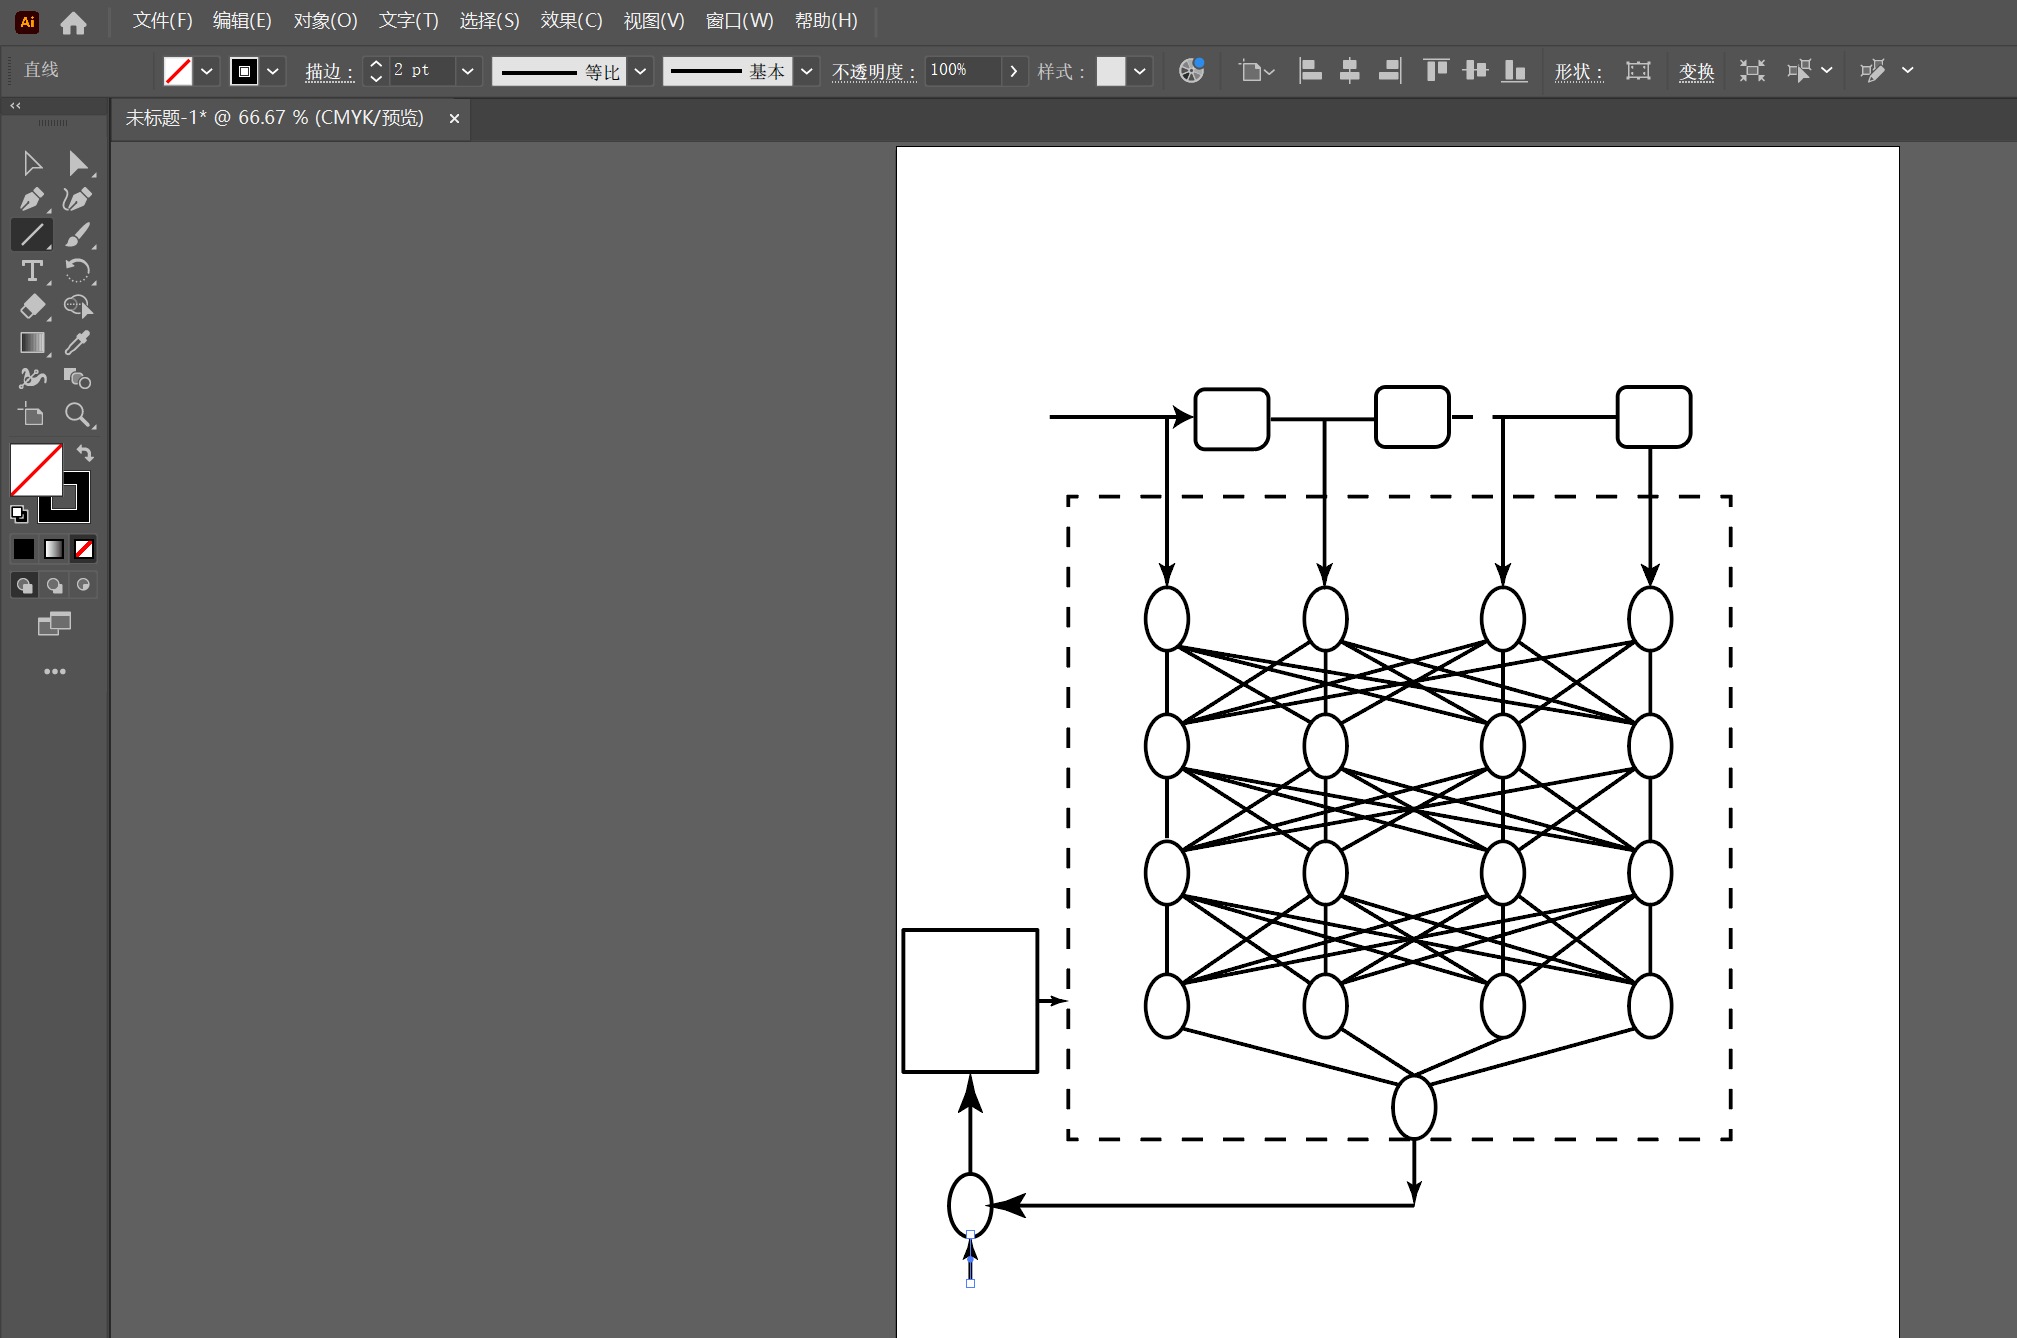
\includegraphics[width=\linewidth]{p6.png}
\section{反思和总结}
\subsection{收获}
这次夏令营让我获得了大量科研实践经验,为我未来的科研和创作奠定了基础,同时,参加夏令营也让我体验到了与前辈和导师一起学习的乐趣,并通过圆桌会议的形式共同进步。
\subsection{存在的疑问}
对我来说,还有很多软件没有掌握更详细的使用方法,比如AI绘图,对于光通信、硅基光电子等理论知识仍然不熟悉,需要了解更多相关知识,还没有掌握科研和创作的实践经验等,在未来,我必须朝着这个方向努力。
\end{document}